\documentclass{beamer}
\usetheme{tokitex}

\usepackage{graphics}
\usepackage{multirow}
\usepackage{tabto}

\usepackage[english,bahasa]{babel}
\newtranslation[to=bahasa]{Section}{Bagian}
\newtranslation[to=bahasa]{Subsection}{Subbagian}

\usepackage{listings, lstautogobble}
\usepackage{color}

\definecolor{dkgreen}{rgb}{0,0.6,0}
\definecolor{gray}{rgb}{0.5,0.5,0.5}
\definecolor{mauve}{rgb}{0.58,0,0.82}

\lstset{frame=tb,
  language=pascal,
  aboveskip=1mm,
  belowskip=1mm,
  showstringspaces=false,
  columns=fullflexible,
  keepspaces=true,
  basicstyle={\small\ttfamily},
  numbers=none,
  numberstyle=\tiny\color{gray},
  keywordstyle=\color{blue},
  commentstyle=\color{dkgreen},
  stringstyle=\color{mauve},
  breaklines=true,
  breakatwhitespace=true,
  autogobble=true
}

\title{Rekursi Lanjutan}
\author{Tim Olimpiade Komputer Indonesia}
\date{}

\begin{document}

\begin{frame}
\titlepage
\end{frame}

\begin{frame}
\frametitle{Pendahuluan}
Melalui dokumen ini, kalian akan:
\begin{itemize}
  \item Mempelajari konsep rekursi yang bercabang.
  \item Belajar merancang fungsi/prosedur rekursif yang lebih sulit.
\end{itemize}
\end{frame}

\section{Fibonacci}
\frame{\sectionpage}

\begin{frame}
\frametitle{Soal: Fibonacci}
Deskripsi:
\begin{itemize}
  \item Pak Dengklek kini beralih untuk mempelajari deret Fibonacci.
  \item Deret fibonacci merupakan deret yang mana suatu anggota adalah penjumlahan dari dua anggota sebelumnya, kecuali dua anggota pertama.
  \item Jika $f_N$ adalah bilangan fibonacci ke-$N$, maka $f_0$ = 0, $f_1$ = 1, dan $f_N$ = $f_{N-1}$ + $f_{N-2}$ untuk $N > 1$
  \item Beberapa bilangan pertama dari deret fibonacci adalah 0, 1, 1, 2, 3, 5, 8, 13, 21, $\dots$
  \item Bantulah Pak Dengklek cari bilangan fibonacci ke-$N$.
  \item Contoh: Bilangan fibonacci ke-6 adalah 8. Perhatikan bahwa indeks dimulai dari 0.
\end{itemize}
\end{frame}

\begin{frame}
\frametitle{Soal: Fibonacci (lanj.) }
Format masukan:
\begin{itemize}
    \item Sebuah baris berisi sebuah bilangan $N$.
\end{itemize}
Format keluaran:
\begin{itemize}
    \item Sebuah baris berisi bilangan fibonacci ke-$N$.
\end{itemize}
Batasan:
\begin{itemize}
    \item $0 \le N \le 20$
\end{itemize}
\end{frame}

\begin{frame}
\frametitle{Solusi}
\begin{itemize}
  \item Bagaimana cara mendapatkan nilai dari dua bilangan fibonacci sebelum bilangan fibonacci ke-$N$?
  \item Apakah kita bisa melakukan rekursi untuk mencari bilangan fibonacci ke-$(N-1)$ dan ke-$(N-2)$?
\end{itemize}
\end{frame}

\begin{frame}
\frametitle{Penjelasan solusi Rekursi}
\textit{Base Case}
\begin{itemize}
  \item Pada batasan soal, nilai $N$ berkisar antara $0$ sampai $20$.
  \item Dari batasan tersebut, kasus terkecil yang sudah pasti diketahui jawabannya adalah $f_0$ dan $f_1$.
  \item Nilai dari $f_0$ = 0 dan $f_1$ = 1, atau dapat dituliskan $f_N = N$, untuk $0 \le N \le 1$.
  \item Jadi $N=0$ dan $N=1$ adalah \textit{base case}.
\end{itemize}
\end{frame}

\begin{frame}
\frametitle{Penjelasan solusi Rekursi (lanj.) }
\textit{Recurrence Relation}
\begin{itemize}
  \item Bagaimana jika $N > 1$?
  \item Seperti yang sudah didefinisikan, $f_N$ = $f_{N-1}$ + $f_{N-2}$ untuk $N > 1$
  \item Contoh: $f_5$ = $f_4$ + $f_3$
  \item Mencari $f_4$ dan $f_3$ sendiri juga memunculkan permasalahan yang lebih kecil, yaitu:
  \begin{itemize}
    \item $f_4 = f_3 + f_2$
    \item $f_3 = f_2 + f_1$ 
  \end{itemize}
  \item Hal ini akan terus diulang tercapai \textit{base case}, yaitu $f_0$ atau $f_1$
  \item Dengan ini, kita menemukan hubungan rekursif dari $f_N$.
\end{itemize}
\end{frame}

\begin{frame}[fragile]
\frametitle{Contoh Solusi: fibonacci\_rekursi.pas}
Perhatikan contoh berikut:
\begin{lstlisting}
   function fibonacci(N: longint): longint;
   begin
     if (N <= 1) then begin
       fibonacci := N;
     end else begin
       fibonacci := fibonacci(N-1) + fibonacci(N-2);
     end;
   end;
\end{lstlisting}
\end{frame}

\begin{frame}[fragile]
\frametitle{Penjelasan solusi rekursi}
Alur eksekusi rekursi dapat dimodelkan dengan pohon rekursi. Berikut adalah contoh pohonnya untuk $f_4$.
\begin{tikzpicture}[level/.style={sibling distance=45mm/#1}]
\node [circle,draw] (z){$f_4$}
  child {node [circle,draw] (a) {$f_3$}
  child {node [circle,draw] (b) {$f_2$}
    child {node [circle,draw] (j) {$f_1$}}
    child {node [circle,draw] (j) {$f_0$}}
    }
  child {node [circle,draw] (g) {$f_1$}}
  }
  child {node [circle,draw] (j) {$f_2$}
    child {node [circle,draw] (k) {$f_1$}}
    child {node [circle,draw] (k) {$f_0$}}
  };
\end{tikzpicture}
\end{frame}

\begin{frame}
\frametitle{Penjelasan solusi rekursi (lanj.)}
Yang terjadi pada program ketika menghitung $f_4$:
\begin {itemize}
  \item Panggil fibonacci(4).
  \item fibonacci(4) akan memeriksa, apakah $N=4$ adalah \textit{base case}.
  \item Ternyata bukan, karena baru $base case$ jika N $\le$ 1.
  \item Dijalankanlah "fibonacci := fibonacci(3) + fibonacci(2)".
  \item Alur rekursi berjalan berurutan, sehingga fibonacci(3) dieksekusi lebih dulu.
\end{itemize}
\end{frame}

\begin{frame}
\frametitle{Penjelasan solusi rekursi (lanj.)}
\begin{itemize}
  \item fibonacci(3) akan menjalankan "fibonacci := fibonacci(2) + fibonacci(1)".
  \item fibonacci(2) akan menjalankan "fibonacci := fibonacci(1) + fibonacci(0)".
  \item Ternyata ketika fibonacci(1), 1 termasuk $base case$ sehingga fibonacci(1) = 1.
  \item Ternyata ketika fibonacci(0), 0 termasuk $base case$ sehingga fibonacci(0) = 0.
  \item Kembali ke fibonacci(2), nilai dari fibonacci(2) menjadi 1 + 0 = 1.
\end{itemize}
\end{frame}

\begin{frame}
\frametitle{Penjelasan solusi rekursi (lanj.)}
\begin {itemize}
  \item Kembali ke fibonacci(3), nilai fibonacci(2) sudah ada nilainya tetapi fibonacci(1) belum sehingga akan dipanggil dan langsung menghasilkan 1 (karena sudah \textit{base case}). Nilai dari fibonacci(3) menjadi 1 + 1 = 2.
  \item Kembali ke fibonacci(4), nilai fibonacci(3) sudah ada nilainya tetapi fibonacci(2) belum sehingga akan dipanggil dan akan menghasilkan 1 (alur yang terjadi sama seperti sebelumnya). Nilai dari fibonacci(4) menjadi 2 + 1 = 3.
\end{itemize}
Tantangan : Cobalah membuat pohon rekursi dan alurnya untuk menghitung $f_5$
\end{frame}

\begin{frame}
\frametitle{Kompleksitas solusi}
\begin {itemize}
   \item Perhatikan pohon rekursi yang sebelumnya. Berapa kali fungsi akan dipanggil?
   \item Setiap pemanggilan fungsi akan bercabang 2 dan kedalaman maksimalnya adalah $N$.
   \item Sebagai pendekatan, bisa dikatakan fungsi dipanggil $2^N$ kali.
   \item Kompleksitasnya menjadi $O(2^{N})$.
\end {itemize}
\end{frame}

\begin{frame}
\frametitle{Masalah}
\begin{itemize}
  \item Perhatikan kembali pohon rekursi yang sebelumnya. Terlihat $f_2$ dihitung dua kali.
  \item Ketika $f_N$ cukup besar, ada banyak fungsi dengan parameter yang sama namun dihitung berkali-kali. Hal ini berakibat program berjalan lambat.
  \item Kita dapat mereduksi kompleksitas rekursi fibonacci menjadi $O(N)$ dengan teknik yang akan kita pelajari pada pemrograman lanjut.
  \item Kita juga bisa membuat solusi $O(N)$ dengan menghitung nilai fibonacci secara iteratif. Dapatkah Anda membuatnya?
\end{itemize}
\end{frame}

\section{Permutasi}
\frame{\sectionpage}


\begin{frame}
\frametitle{Soal: Permutasi}
Deskripsi:
\begin{itemize}
  \item Pak Dengklek lupa password akun TLX-nya!
  \item Yang ia ingat hanyalah passwordnya terdiri dari $N$ angka, dan mengandung masing-masing angka dari $1$ sampai $N$.
  \item Misalnya $N=3$, bisa jadi password Pak Dengklek adalah 123, 132, 312, dst
  \item Bantu Pak Dengklek menuliskan semua kemungkinan passwordnya!
\end{itemize}
\end{frame}

\begin{frame}
\frametitle{Soal: Permutasi (lanj.) }
Format masukan:
\begin{itemize}
    \item Sebuah baris berisi sebuah bilangan $N$.
\end{itemize}
Format keluaran:
\begin{itemize}
    \item Beberapa baris yang merupakan semua kemungkinan password, satu pada setiap barisnya.
    \item Urutkan keluaran secara leksikografis (seperti pada kamus).
\end{itemize}
Batasan:
\begin{itemize}
    \item $1 \le N \le 8$
\end{itemize}
\end{frame}

\begin{frame}[fragile]
\frametitle{Soal: Permutasi (lanj.) }
Contoh masukan:
\begin{lstlisting}
3
\end{lstlisting}

\vfill

Contoh keluaran:
\begin{lstlisting}
123
132
213
231
312
321
\end{lstlisting}
\end{frame}

\begin{frame}[fragile]
\frametitle{Solusi}
\begin{itemize}
  \item Sebelum merancang solusi untuk persoalan sebenarnya, mari kita sederhanakan persoalan.
  \item Misalkan digit-digit boleh berulang, sehingga untuk $N=3$, keluarannya adalah:
  
  \begin{lstlisting}
  111
  112
  113
  121
  122
  123
  131
  ...
  333
  \end{lstlisting}
\end{itemize}
\end{frame}

\begin{frame}[fragile]
\frametitle{Solusi (lanj.)}
\begin{itemize}
  \item Jika $N$ selalu 3, terdapat solusi iteratif yang sederhana:
  
  \begin{lstlisting}
  for i := 1 to 3 do begin
    for j := 1 to 3 do begin
      for k := 1 to 3 do begin
        writeln(i, j, k);
      end;
    end; 
  end;
  \end{lstlisting}
\end{itemize}
\end{frame}

\begin{frame}[fragile]
\frametitle{Solusi (lanj.)}
\begin{itemize}
  \item Namun bagaimana jika $N=2$? Atau $N=4$?
  \item Kedalaman \textbf{for loop} tidak bisa diatur untuk memenuhi kebutuhan $N$ yang beragam!
  \item Untuk itu, solusi rekursif lebih mudah digunakan untuk persoalan yang disederhanakan ini.
\end{itemize}
\end{frame}

\begin{frame}[fragile]
\frametitle{Ide Rekursif}
\begin{itemize}
  \item Setiap kedalaman \textbf{loop} bisa diwujudkan oleh sebuah pemanggilan rekursif.
  
  \begin{figure}
    \centering 
    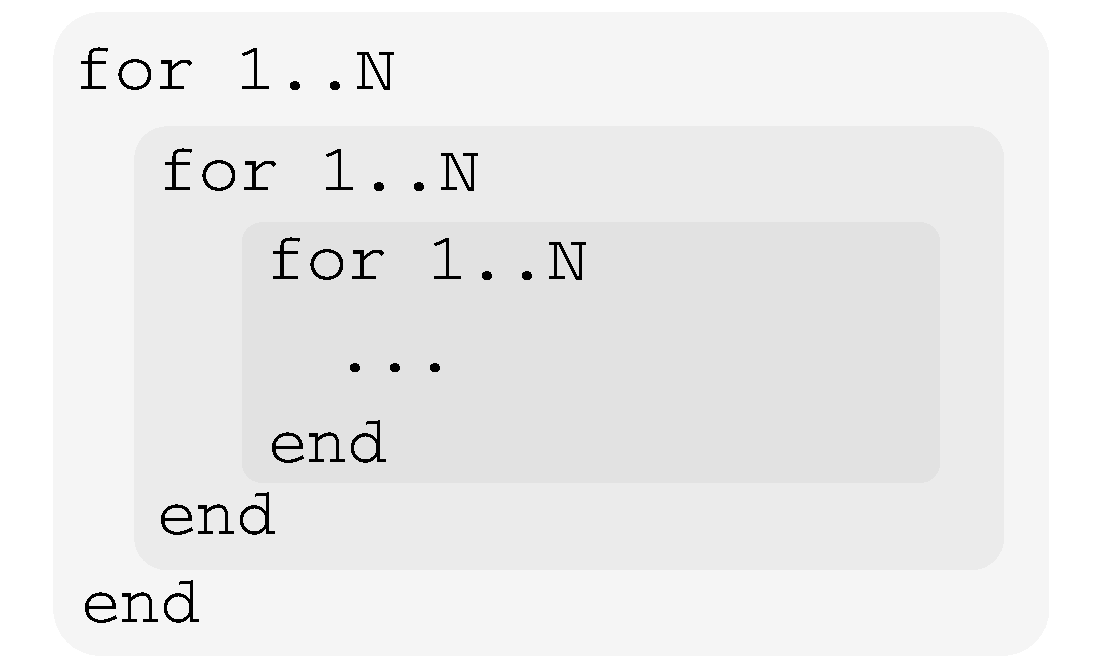
\includegraphics[width=6cm]{asset/lapis.pdf}
  \end{figure}
  
  \item Dengan menambahkan parameter "kedalaman" pada pemanggilan rekursif, kedalaman dari \textbf{loop} dapat diatur.
\end{itemize}
\end{frame}

\begin{frame}[fragile]
\frametitle{Ide Rekursif (lanj.)}
\begin{lstlisting}
procedure tulis(kedalaman: longint);
var
  i: longint;
begin
  if (kedalaman > N) then begin
    (* cetak password *)
    ...
  end else begin
    (* masuk ke lapisan lebih dalam *)
    for i := 1 to N do begin
      tulis(kedalaman + 1);
    end;
  end;
end;
\end{lstlisting}
\end{frame}

\begin{frame}[fragile]
\frametitle{Ide Rekursif (lanj.)}
\begin{itemize}
  \item Prosedur \textbf{tulis} dapat dipanggil dengan perintah:
  \begin{lstlisting}
  tulis(1);
  \end{lstlisting}
  
  \item Nilai \textbf{kedalaman} akan terus bertambah selama kedalaman saat ini belum mencapai $N$. 
  \item Hal ini menjadi memicu pemanggilan rekursif lebih dalam.
  \item Setelah \textbf{kedalaman} melebihi $N$, artinya tidak perlu lagi menambah "lapisan \textbf{loop}", sehingga dicapai \textit{base case} dan dicetak password. 
\end{itemize}
\end{frame}

\begin{frame}[fragile]
\frametitle{Ide Rekursif (lanj.)}
\begin{itemize}
  \item Masalah berikutnya adalah bagaimana mencatat password yang sejauh ini telah dibentuk.
  \item Salah satu solusinya adalah membuat array global yang mencatat digit password dari 1 sampai \textbf{kedalaman}.
  \item Ketika \textit{base case} tercapai, kita bisa mencetak isi array tersebut.
  \item Kita namakan array tersebut \textbf{catat}.
\end{itemize}
\end{frame}

\begin{frame}[fragile]
\frametitle{Ide Rekursif (lanj.)}
\begin{lstlisting}
procedure tulis(kedalaman: longint);
var
  i: longint;
begin
  if (kedalaman > N) then begin
    for i := 1 to N do begin 
      write(catat[i]);       (* cetak *)
    end;
    writeln;
  end else begin
    for i := 1 to N do begin
      catat[kedalaman] := i; (* catat di sini *)
      tulis(kedalaman + 1);
    end;
  end;
end;
\end{lstlisting}
\end{frame}

\begin{frame}[fragile]
\frametitle{Solusi untuk Permutasi}
\begin{itemize}
  \item Kita berhasil menyelesaikan masalah yang disederhanakan, saatnya menarik solusi tersebut ke masalah sebenarnya.
  \item Perbedaan dari masalah yang baru kita selesaikan dengan yang sebenarnya adalah: tidak boleh ada digit yang berulang.
  \item Sebagai contoh, 122, 212, 311 bukan password yang benar, sementara 123, 213, dan 321 merupakan password yang benar.
  \item Artinya, jika kita bisa menghindari mencetak password dengan digit berulang, masalah selesai.
\end{itemize}
\end{frame}

\begin{frame}[fragile]
\frametitle{Menghindari Digit Berulang}
Solusi yang mungkin:
\begin{itemize}
  \item Sebelum mencetak, periksa apakah ada digit yang berulang.
  \item Sebelum melakukan pemanggilan rekursif yang lebih dalam, periksa apakah ada digit berulang yang tercatat.
\end{itemize}   
\end{frame}

\begin{frame}[fragile]
\frametitle{Menghindari Digit Berulang (lanj.)}
\begin{itemize}
  \item Solusi pertama kurang cocok digunakan.
  \item Misalkan untuk $N=8$, dan kedalaman saat ini adalah 2. 
  \item Diketahui bahwa array \textbf{catat} sejauh ini berisi [1, 1, ...].
  \item Tidak ada gunanya untuk meneruskan pemanggilan rekursif lebih dalam, sebab kemungkinan ini sudah pasti tidak dicetak (ada digit '1' berulang).
\end{itemize}   
\end{frame}

\begin{frame}
\frametitle{Menghindari Digit Berulang (lanj.)}
\begin{itemize}
  \item Mengindari perulangan digit sebelum pemanggilan rekursif lebih efisien untuk digunakan.
  \item Oleh karena itu kita akan menggunakan cara kedua.
  \item Hal ini dapat dilakukan dengan menandai digit-digit yang sudah pernah digunakan, dan jangan mencatat digit-digit tersebut.
\end{itemize}   
\end{frame}

\begin{frame}
\frametitle{Menghindari Digit Berulang (lanj.)}
\begin{itemize}
  \item Kita akan menggunakan array global bertipe \textbf{boolean}, yaitu \textbf{pernah}.
  \item Awalnya, seluruh isi array \textbf{pernah} adalah \textbf{false}.
  \item \textbf{pernah[i]} bernilai \textbf{true} jika digit \textbf{i} berada di dalam array \textbf{catat}.
  \item Setiap sebelum masuk ke kedalaman rekursif berikutnya, periksa apakah digit yang akan digunakan sudah pernah digunakan.
  \item Jika belum pernah, baru boleh digunakan.
\end{itemize}   
\end{frame}

\begin{frame}[fragile]
\frametitle{Implementasi}
\begin{lstlisting}
procedure tulis(kedalaman: longint);
var
  i: longint;
begin
  if (kedalaman > N) then begin
    (* bagian mencetak *)
  end else begin
    for i := 1 to N do begin
      if (not pernah[i]) then begin (* i belum pernah? *)
        pernah[i] := true;          (* gunakan *)
        catat[kedalaman] := i;      (* catat *)
        tulis(kedalaman + 1);
        pernah[i] := false;         (* selesai *)
      end; 
    end;
  end;
end;
\end{lstlisting}
\end{frame}
  
\begin{frame}
\frametitle{Menghindari Digit Berulang (lanj.)}
\begin{itemize}
  \item Setelah perintah "tulis(kedalaman + 1)", nilai \textbf{pernah[i]} perlu dikembalikan menjadi \textbf{false}.
  \item Sebab setelah keluar dari pemanggilan rekursif tersebut, digit \textbf{i} dianggap tidak lagi ada pada \textbf{catat}.
  \item Namun digit \textbf{i} bisa saja digunakan untuk beberapa pemanggilan rekursif ke depannya.
  \item Dengan cara ini, kita memastikan tidak ada digit berulang yang dicetak.
\end{itemize}   
\end{frame}

\begin{frame}[fragile]
\frametitle{Kompleksitas}
\begin{itemize}
  \item Jika $N=3$, maka berikut pohon rekursif yang menggambarkan pemilihan \textbf{i} untuk setiap pemanggilan:
\end{itemize}   
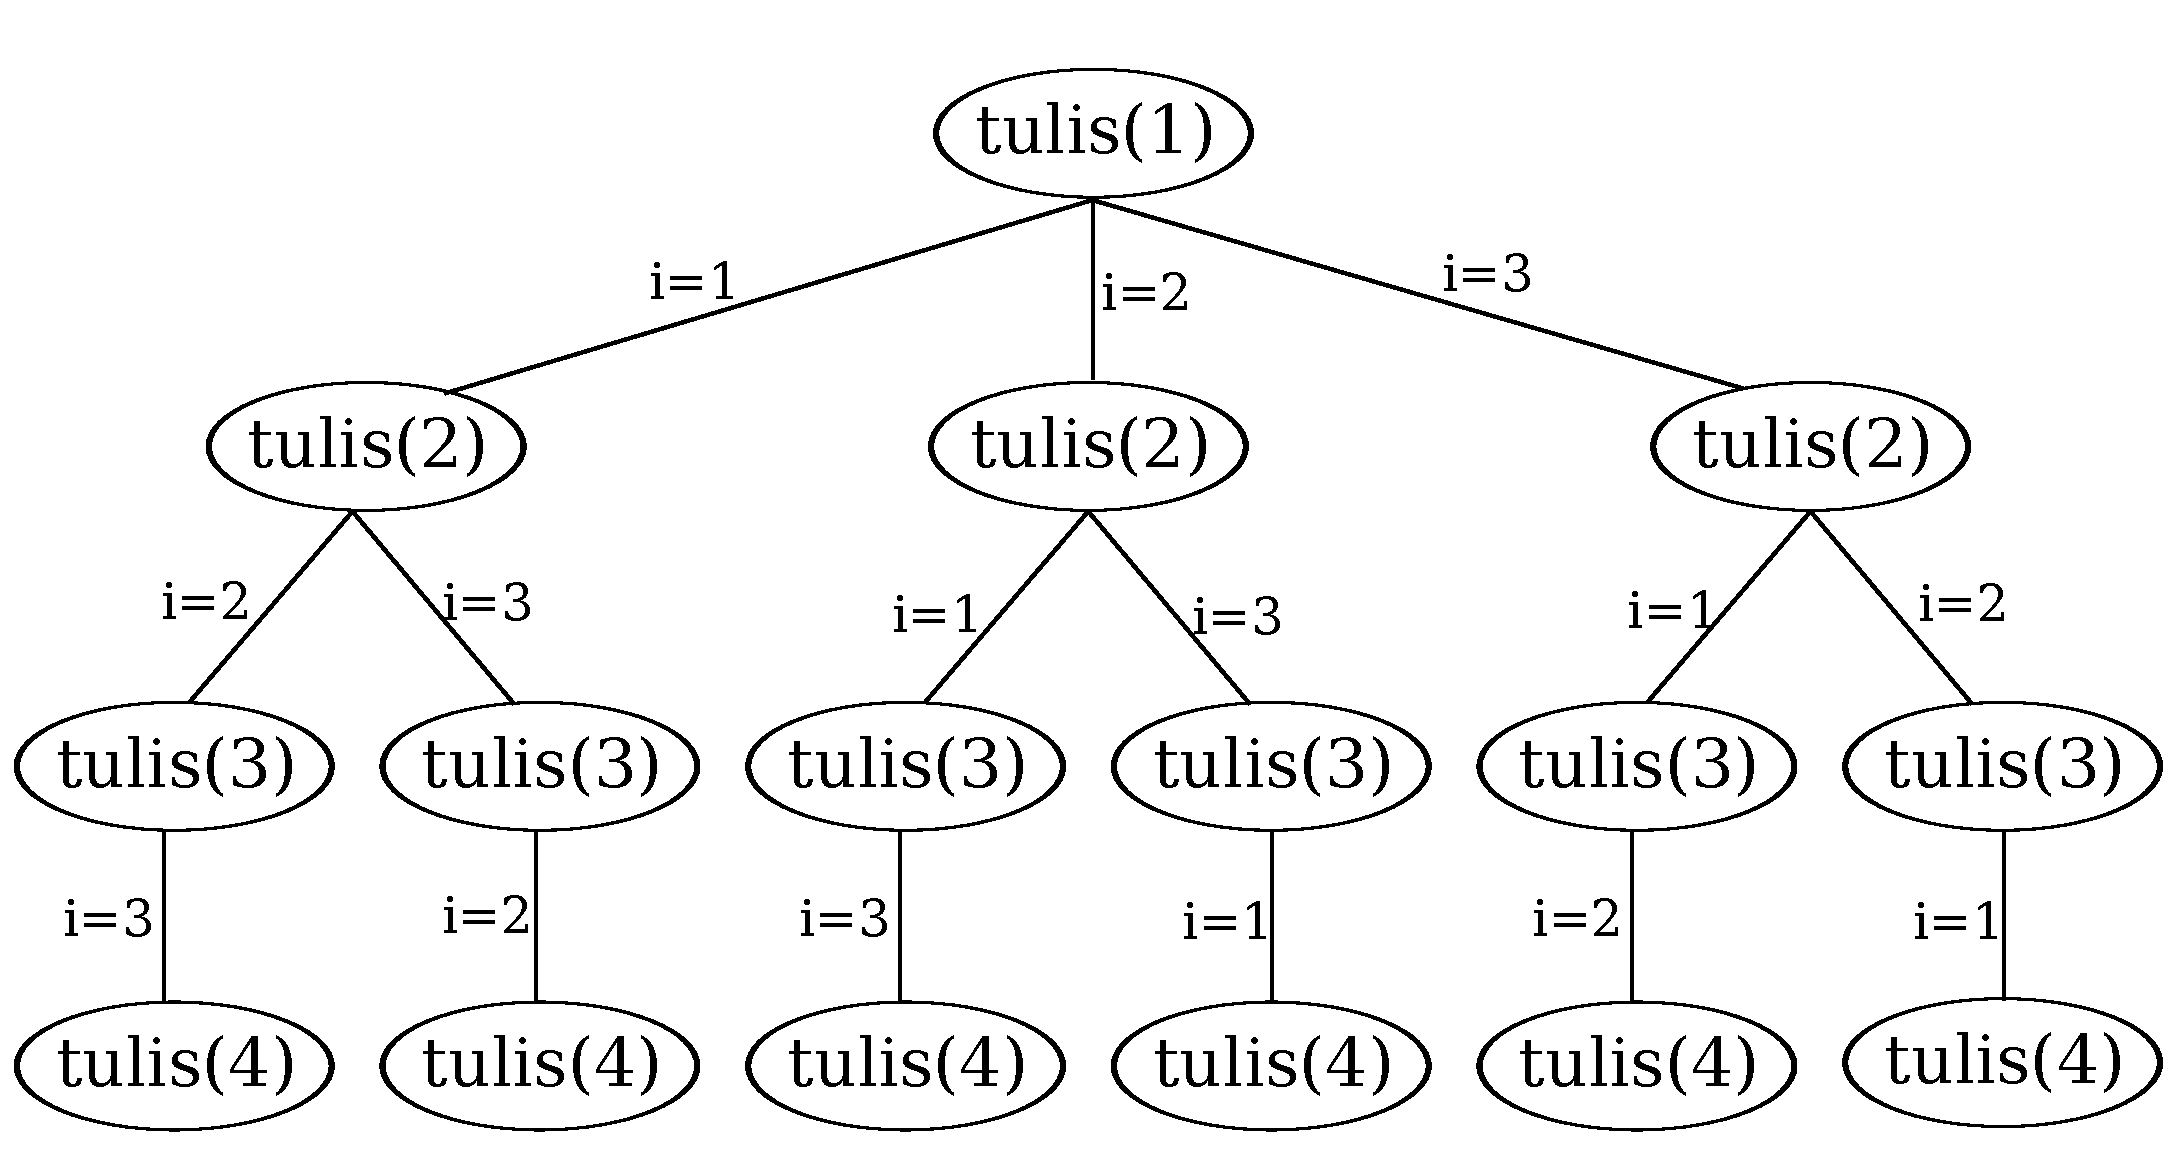
\includegraphics[width=11cm]{asset/permutasi.pdf}
\end{frame}

\begin{frame}[fragile]
\frametitle{Kompleksitas}
\begin{itemize}
  \item Dapat diperhatikan bahwa pada kedalaman pertama, terdapat $N$ cabang rekursif.
  \item Pada kedalaman kedua, terdapat $N-1$ cabang rekursif.
  \item Seterusnya hingga kedalaman terakhir yang tidak lagi bercabang.
  \item Kompleksitasnya adalah $N \times (N-1) \times (N-2) \times ... \times 1$, atau dengan kata lain $O(N!)$.
\end{itemize}   
\end{frame}

\begin{frame}
\frametitle{Penutup}
\begin{itemize}
  \item Rekursi merupakan topik yang luas untuk dibicarakan.
  \item Jika Anda belum terbiasa dengan berpikir rekursif, maka latihan yang banyak adalah solusinya.
  \item Selamat berlatih dengan soal-soal yang ada!
\end{itemize}   
\end{frame}

\end{document}
